% !Mode:: "TeX:UTF-8"
% !TEX program = xelatex
\documentclass[a4paper]{article}
\usepackage{amsmath}
\usepackage{amssymb}
\usepackage{ctex}
%\usepackage{braket}
%\usepackage[european]{circuitikz}
\usepackage{multirow}
\usepackage{float}
\usepackage{graphicx}
\usepackage{geometry}
\geometry{left=2.5cm,right=2.5cm,bottom=2.5cm,top=2.5cm}
\title{近代物理实验报告2.3:等离子体分析}
\author{林杨\quad 211840092\quad 物理学院}
\date{2024年9月26日}
\begin{document}
\maketitle
\bibliographystyle{unsrt}
%--------main-body------------

\section{引言}
等离子体作为物质的第四态在宇宙中普遍存在。在实验室中对等离子体的研究是从气体放电开始的。朗缪尔(I. Langmuir)和汤克斯(L. Tonks)首先引入“等离子体”这个名称。近年来等离子体物理学有了较快发展,并被应用到电力工业、电子工业、金属加工和广播通讯等部门,特别是等离子体的研究,为利用受控热核反应,解决能源问题提供了诱人的前景。

\section{实验目的}
\begin{enumerate}
\item 了解气体放电中等离子体的特性。
\item 利用等离子体诊断技术测定等离子体的一些基本参量。
\end{enumerate}

\section{实验仪器}
等离子体物理实验组合仪、接线板、等离子体放电管、亥姆霍兹线圈。

\section{实验原理}
\subsection{等离子体及其物理特性}
等离子体(又称等离子区)定义为包含大量正负带电粒子、而又不出现净空间电荷的电离气体。也就是说,其中正负电荷密度相等,整体上呈现电中性。等离子体可分为等温等离子体和不等温等离子体,一般气体放电产生的等离子体属于不等温等离子体。

等离子体有一系列不同于普通气体的特性:
\begin{enumerate}
\item 高度电离,是电和热的良导体,具有比普通气体大几百倍的比热容。
\item 带正电的和带负电的粒子密度几乎相等。
\item 宏观上是电中性的。
\end{enumerate}
虽然等离子体宏观上是电中性的,但是由于电子的热运动,等离子体局部会偏离电中性,电荷之间的库伦相互作用,使这种偏离电中性的范围不能无限扩大,最终使电中性得以恢复。偏离电中性的区域最大尺度称为德拜长度$\lambda_D$,当系统尺度L$>\lambda_D$时,系统呈现电中性,当L$<\lambda_D$时,系统可能出现非电中性。
\subsection{等离子体的主要参量}
描述等离子体的一些主要参量为:
\begin{enumerate}
\item 电子温度$T_e$。它是等离子体的一个主要参量,因为在等离子体中电子碰撞电离是主要的,而电子碰撞电离与电子的能量有直接关系,即与电子温度相关联。
\item 带电粒子密度。电子密度为$n_e$,正离子密度为$n_i$,在等离子体中$n_e\approx n_i$。
\item 轴向电场强度$E_L$。表征为维持等离子体的存在所需的能量。
\item 电子平均动能$\bar{E_e}$。
\item 空间电位分布。
\end{enumerate}
此外,由于等离子体中带电粒子间的相互作用是长程的库仑力,使它们在无规则的热运动之外,能产生某些类型的集体运动,如等离子振荡,其振荡频率$f_p$称为朗缪尔频率或等离子体频率。电子振荡时辐射的电磁波称为等离子体电磁辐射。
\subsection{稀薄气体产生的辉光放电}
本实验研究的是辉光放电等离子体。

辉光放电是气体导电的一种形态。当放电管内的压强保持在10$\sim$10$^2$Pa时,在两电极上加高电压,就能观察到管内有放电现象。辉光分为明暗相间的8个区域。8个区域的名称为(1)阿斯顿区,(2)阴极辉区,(3)阴极暗区,(4)负辉区,(5)法拉第暗区,(6)正辉区(即正辉柱),(7)阳极暗区,(8)阴极辉区。
\begin{figure}[!h]
\centering
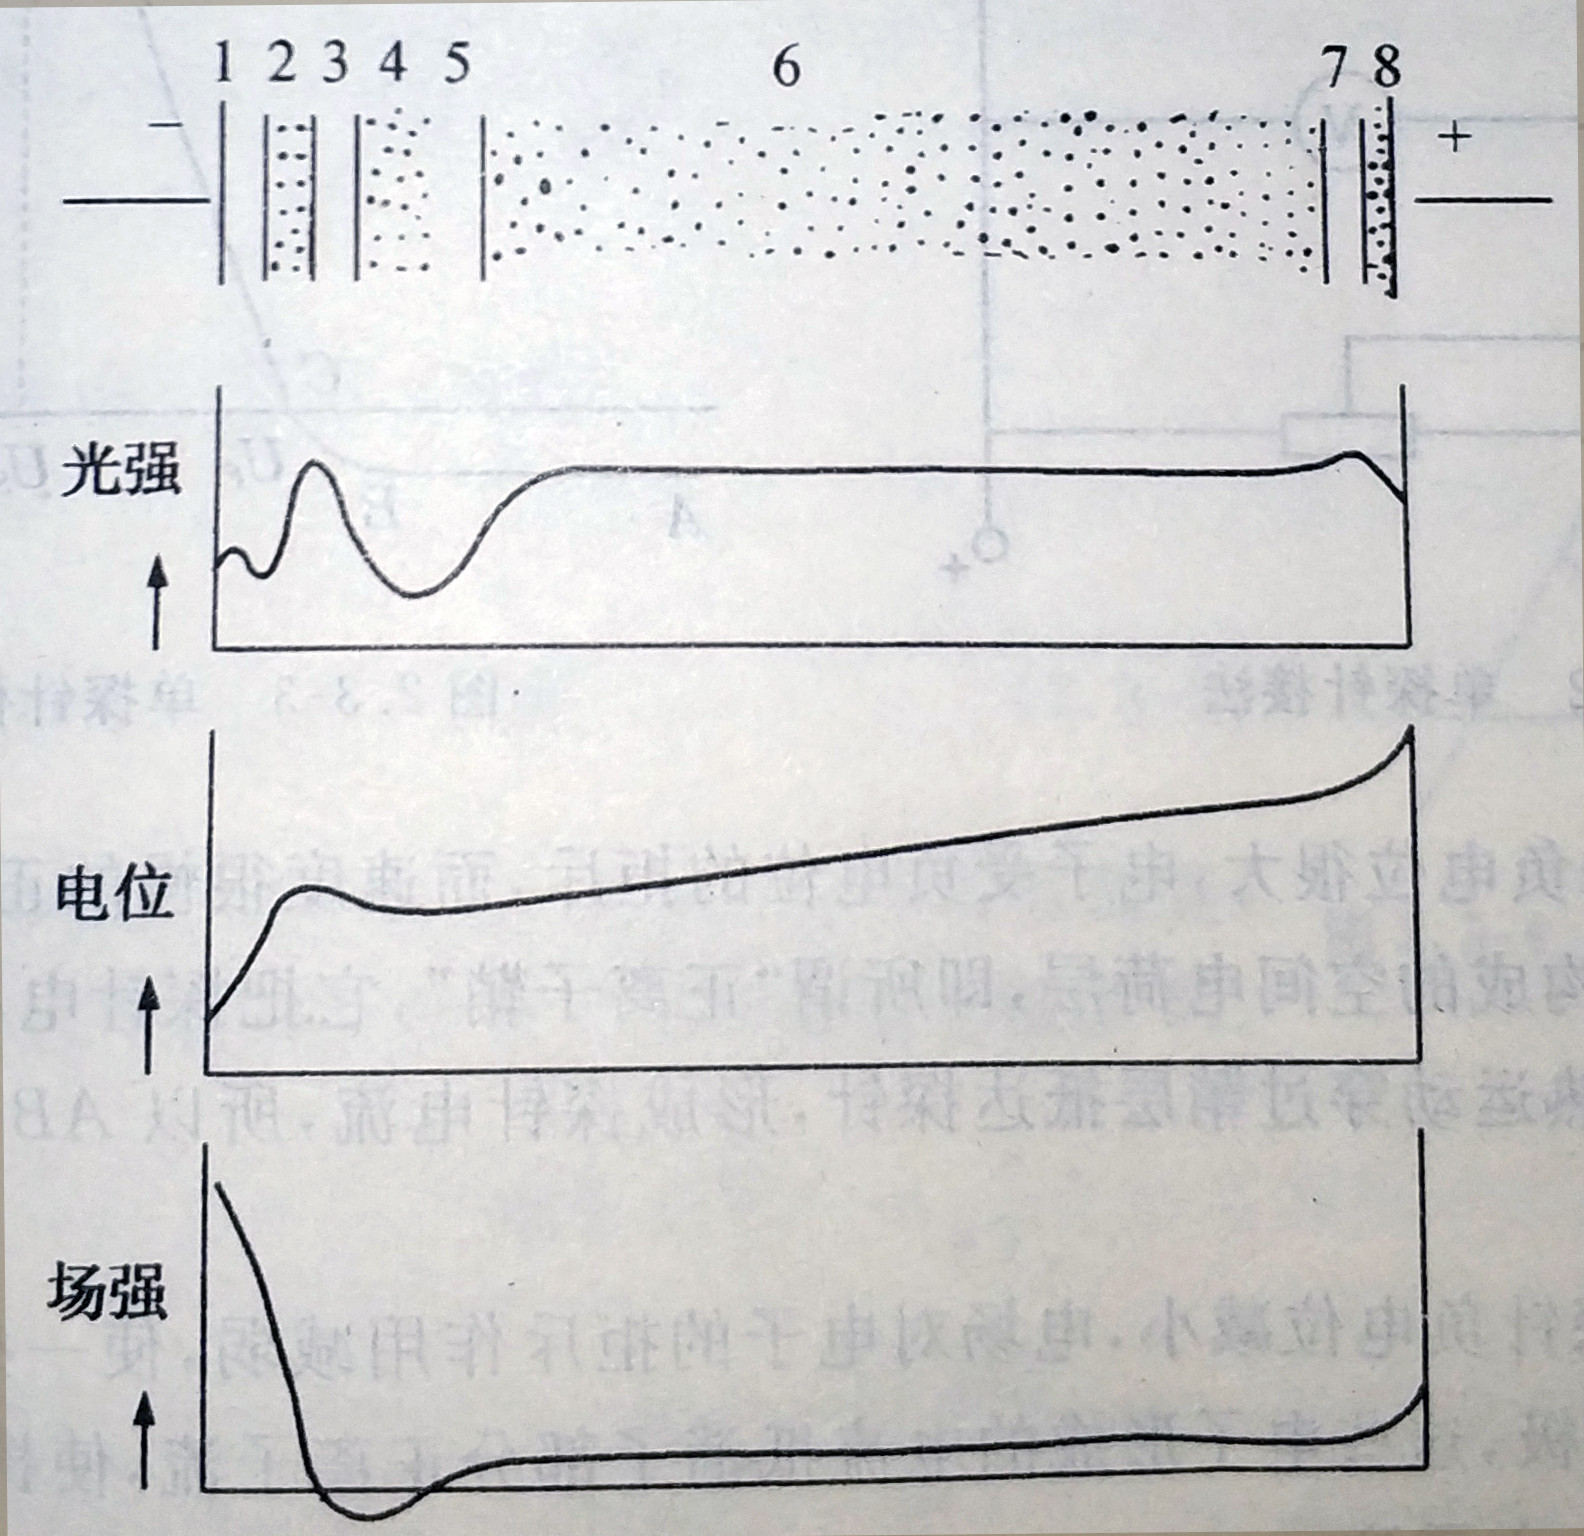
\includegraphics[width=0.6\textwidth]{fig/fig1.jpg}\\
\caption{辉光放电的光强、电位和场强的分布}\label{fig1}
\end{figure}

如图(\ref{fig1})所示,其中正辉区是我们感兴趣的等离子区。其特征是:气体高度电离;电场强度很小,且沿轴向有恒定值。这使得其中带电粒子的无规则热运动胜过它们的定向运动。所以它们基本上遵从麦克斯韦速度分布律。由其具体分布可得到一个相应的温度,即电子温度。但是,由于电子质量小,它在跟离子或原子作弹性碰撞时能量损失很小,所以电子的平均动能比其他粒子的大得多。这是一种非平衡状态。因此,虽然电子温度很高(约为105K),但放电气体的整体温度并不明显升高,放电管的玻璃壁并不软化。
\subsection{等离子体诊断}
测试等离子体的方法被称为诊断。等离子体诊断有(1)探针法,(2)霍尔效应法,(3)微波法,(4)光谱法等。本次实验中采用探针法。探针法分单探针法和双探针法。
\subsubsection{单探针法}
探针是封入等离子体中的一个小的金属电极(其形状可以是平板形、圆柱形、球形),其接法如图(\ref{fig2})所示。
\begin{figure}[!h]
\begin{minipage}{0.48\textwidth}
\begin{center}
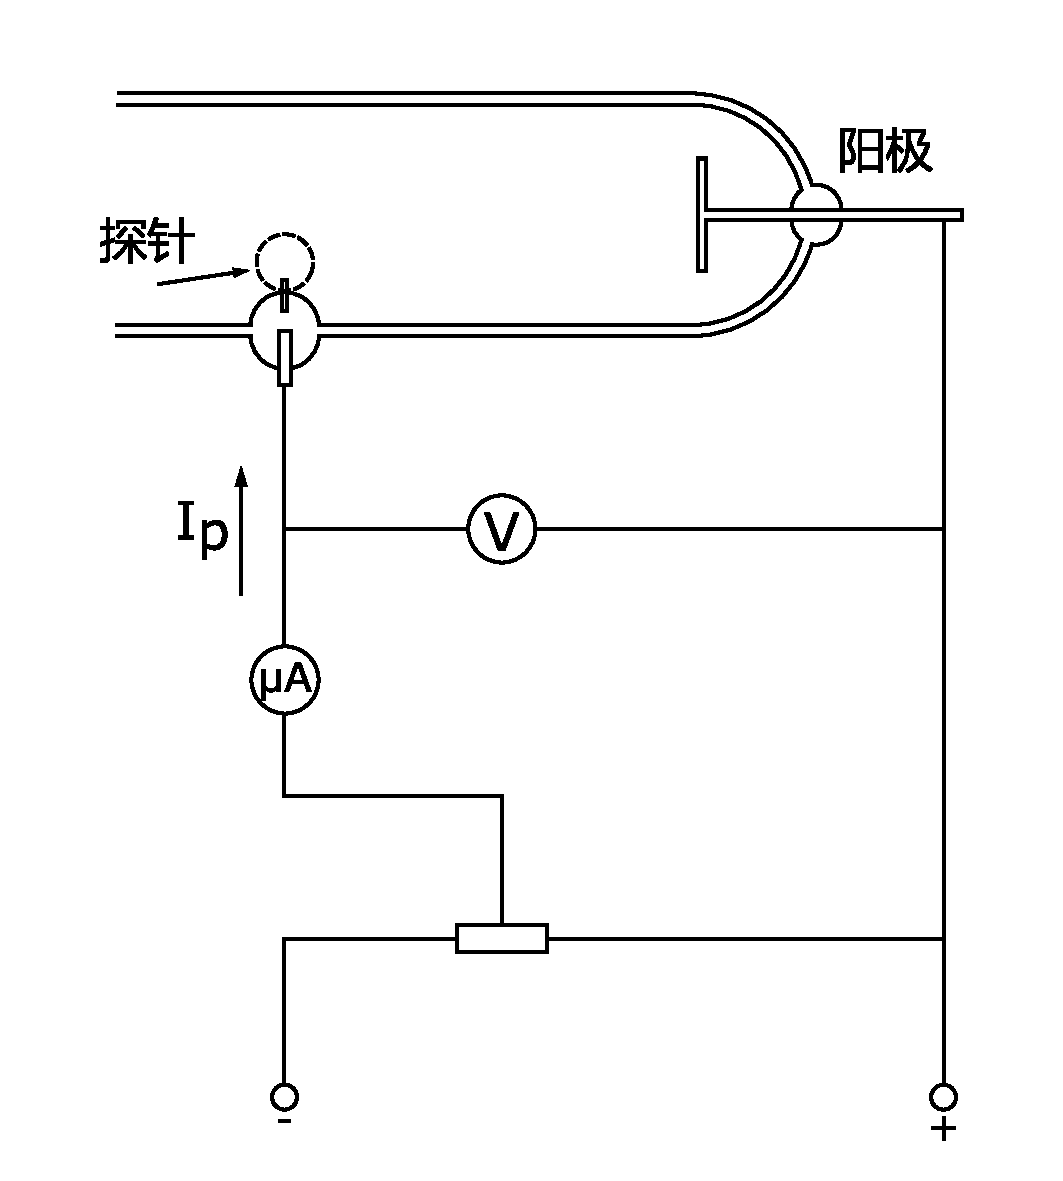
\includegraphics[width=0.9\textwidth]{fig/fig2.pdf}\\
\caption{单探针接法}\label{fig2}
\end{center}
\end{minipage}
\begin{minipage}{0.48\textwidth}
\begin{center}
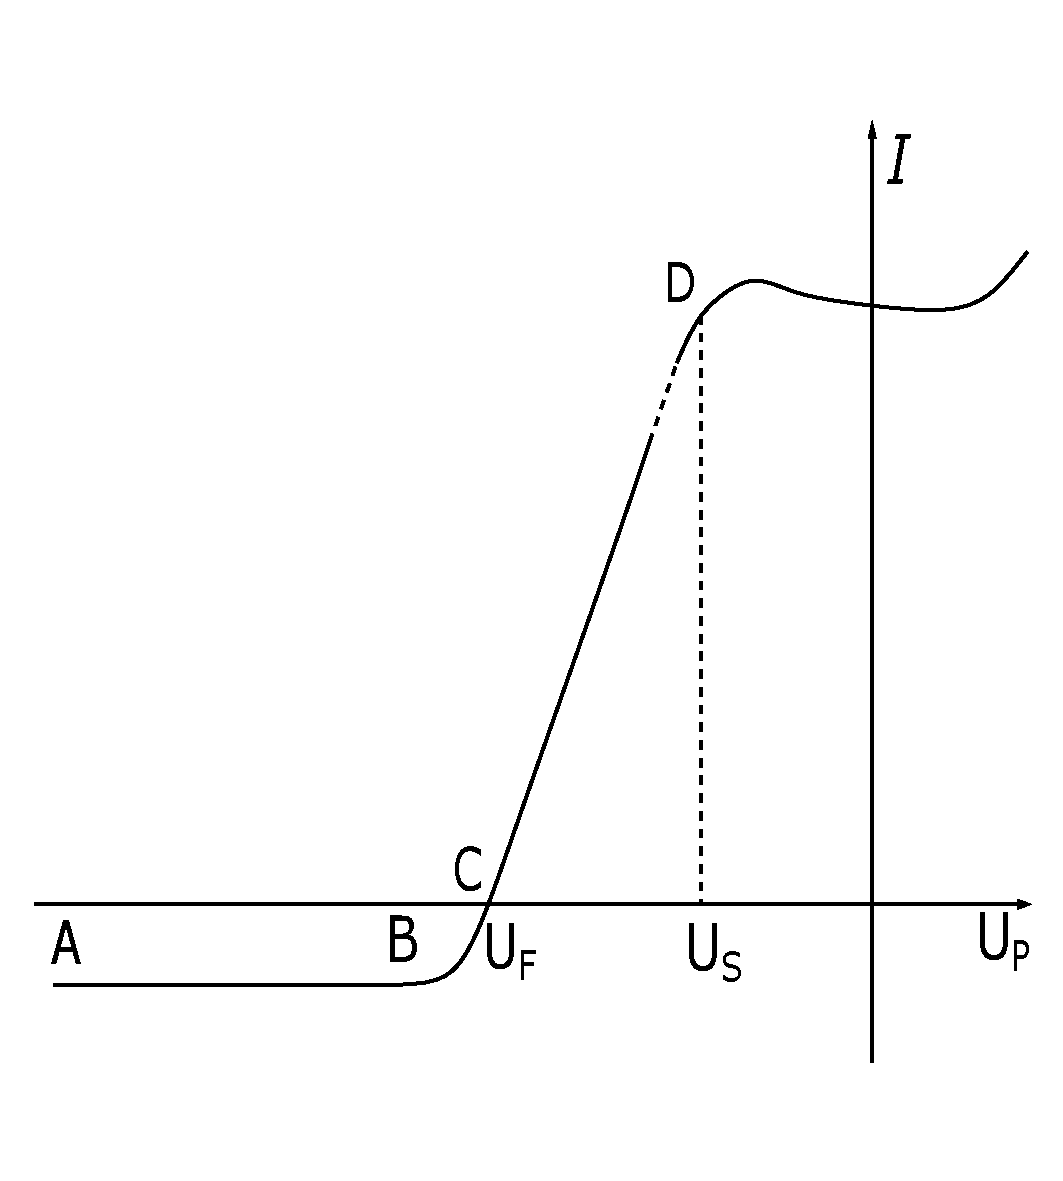
\includegraphics[width=0.9\textwidth]{fig/fig3.pdf}\\
\caption{单探针伏安特性}\label{fig3}
\end{center}
\end{minipage}
\end{figure}

以放电管的阳极或阴极作为参考点,改变探针电位,测出相应的探针电流,得到探针电流与其电位之间的关系,即探针伏安特性曲线,如图(\ref{fig3})所示。对此曲线的解释为:

在AB段,探针的负电位很大,电子受负电位的排斥,而速度很慢的正离子被吸向探针,在探针周围形成正离子构成的空间电荷层,即所谓“正离子鞘”,它把探针电场屏蔽起来。等离子区中的正离子只能靠热运动穿过鞘层抵达探针,形成探针电流,所以AB段为正离子流,这个电流很小。

过了B点,随着探针负电位减小,电场对电子的拒斥作用减弱,使一些快速电子能够克服电场拒斥作用,抵达探极,这些电子形成的电流抵消了部分正离子流,使探针电流逐渐下降,所以BC段为正离子流加电子流。

到了C点,电子流刚好等于正离子流,互相抵消,使探针电流为零。此时探针电位就是悬浮电位$U_F$。

继续减小探极电位绝对值,到达探极电子数比正离子数多得多,探极电流转为正向,并且迅速增大,所以CD段为电子流加离子流,以电子流为主。

当探极电位$U_p$和等离子体的空间电位$U_s$相等时,正离子鞘消失,全部电子都能到达探极,这对应于曲线上的D点。此后电流达到饱和。如果$U_p$进一步升高,探极周围的气体也被电离,使探极电流又迅速增大,甚至烧毁探针。

由单探针法得到的伏安特性曲线,可求得等离子体的一些主要参量。

对于曲线的CD段,由于电子受到减速电位($U_p$-$U_s$)的作用,只有能量比e($U_p$-$U_s$)大的那部分电子能够到达探针。假定等离子区内电子的速度服从麦克斯韦分布,则减速电场中靠近探针表面处的电子密度$n_e$,按玻耳兹曼分布应为
\begin{equation}
n_e = n_0e^{\frac{e(U_p-U_s)}{k_BT_e}}\label{eq1}
\end{equation}
式中$n_0$为等离子区中的电子密度,$T_e$为等离子区中的电子温度,$k_B$为玻耳兹曼常数。在电子平均速度为$v_e$时,在单位时间内落到表面积为S的探针上的电子数为:
\begin{equation}
N_e = \frac{1}{4}n_e\bar{v_e}S\label{eq2}
\end{equation}
得探针上的电子电流
\begin{equation}
I = N_ee = \frac{1}{4}n_e\bar{v}Se = I_0e^{\frac{e(U_p-U_s)}{k_BT_e}}\label{eq3}
\end{equation}
其中
\begin{equation}
I_0 = \frac{1}{4}n_0\bar{v_e}Se\label{eq4}
\end{equation}
\begin{figure}[!h]
\centering
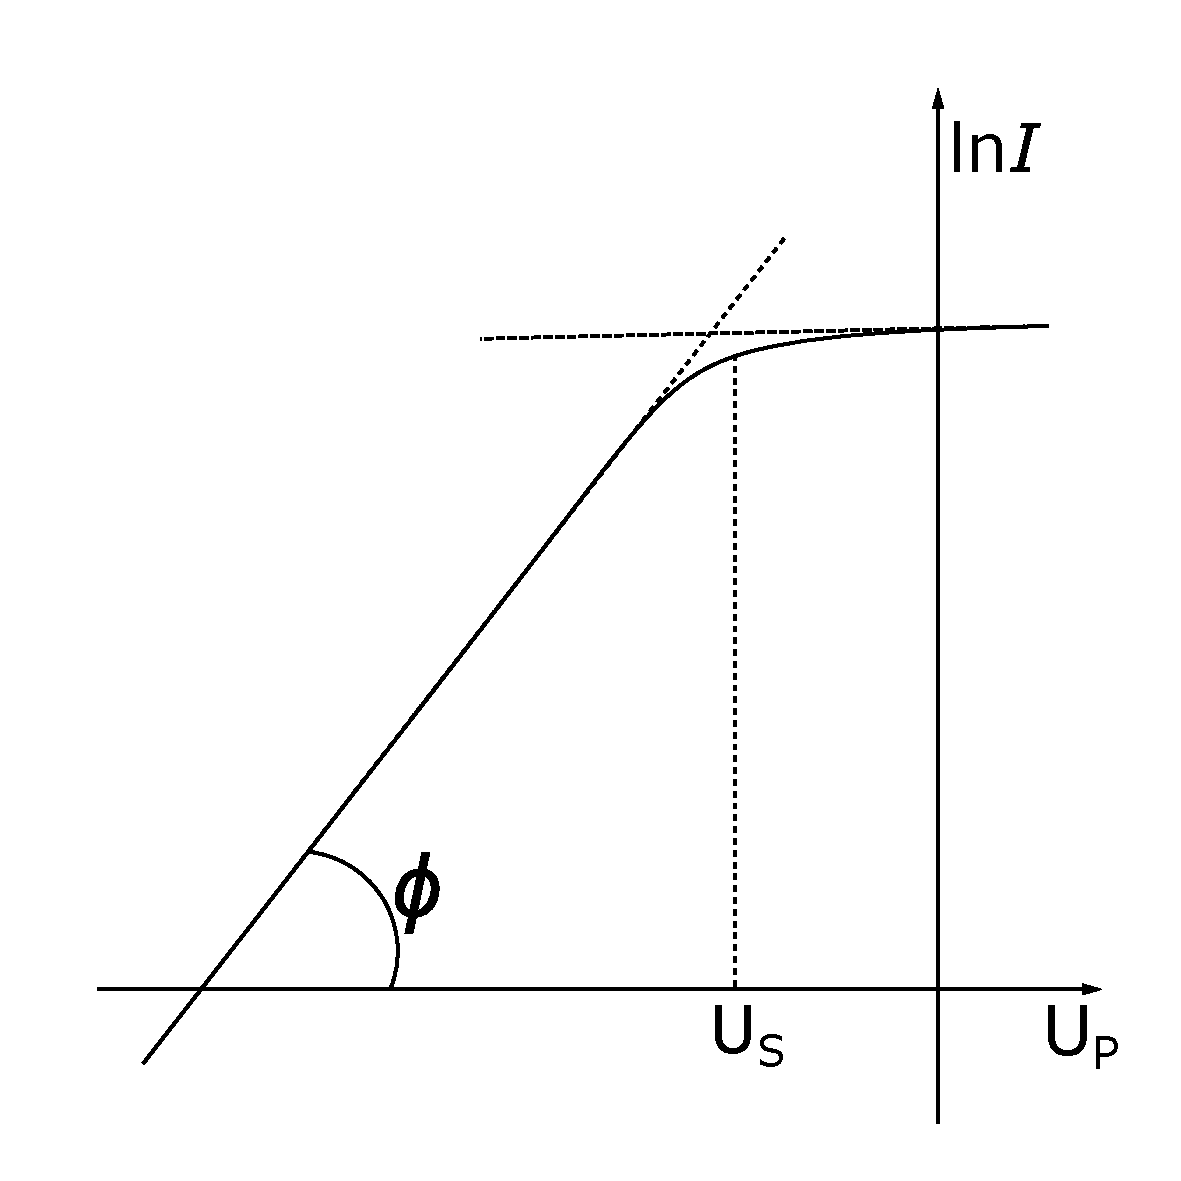
\includegraphics[width=0.4\textwidth]{fig/fig4.pdf}\\
\caption{单探针的半对数曲线}\label{fig4}
\end{figure}

对式(\ref{eq3})取对数
\begin{equation*}
\text{ln}I = \text{ln}I_0 - \cfrac{eU_s}{k_BT_e} + \cfrac{eU_p}{k_BT_e}
\end{equation*}
其中
\begin{equation*}
\text{ln}I_0 - \cfrac{eU_s}{k_BT_e} = \text{常数}
\end{equation*}
故
\begin{equation}
\text{ln}I = \cfrac{eU_p}{k_BT_e} + \text{常数}\label{eq5}
\end{equation}
可见电子电流的对数与探针电位呈线性关系。作半对数曲线,如图(\ref{fig4})所示,由直线部分的斜率$\tan\phi$,可决定电子温度$T_e$:
\begin{equation*}
\tan\phi = \cfrac{\text{ln}I}{U_p} = \cfrac{e}{k_BT_e}
\end{equation*}
\begin{equation}
T_e = \cfrac{e}{k_B\tan\phi} = \cfrac{\text{11600}}{\tan\phi}\label{eq6}
\end{equation}
若取以10为底的对数,则常数11600应改为5040。

电子平均动能$\bar{E_e}$和平均速度$\bar{v_e}$分别为:
\begin{eqnarray}
\bar{E_e} &=& \frac{3}{2}k_BT_e\label{eq7}\\
\bar{v_e} &=& \sqrt{\cfrac{8k_BT_e}{\pi m_e}}\label{eq8}
\end{eqnarray}
式中$m_e$为电子质量。

由式(\ref{eq4})可求得等离子区中的电子密度:
\begin{equation}
n_e = \cfrac{4I_0}{eS\bar{v_e}} = \cfrac{I_0}{eS}\sqrt{\cfrac{2\pi m_e}{k_BT_e}}\label{eq9}
\end{equation}
式中$I_0$为$U_p = U_s$时的电子电流,S为探针裸露在等离子区中的表面积。
\subsubsection{双探针法}
单探针法有一定的局限性,因为探针的电位要以放电管的阳极或阴极电位作为参考点,而且一部分放电电流会对探极电流有所贡献,造成探极电流过大和特性曲线失真。

双探针法是在放电管中装两根探针,相隔一段距离$l$。双探针法的伏安特性曲线如图(\ref{fig5})所示。
\begin{figure}[!h]
\centering
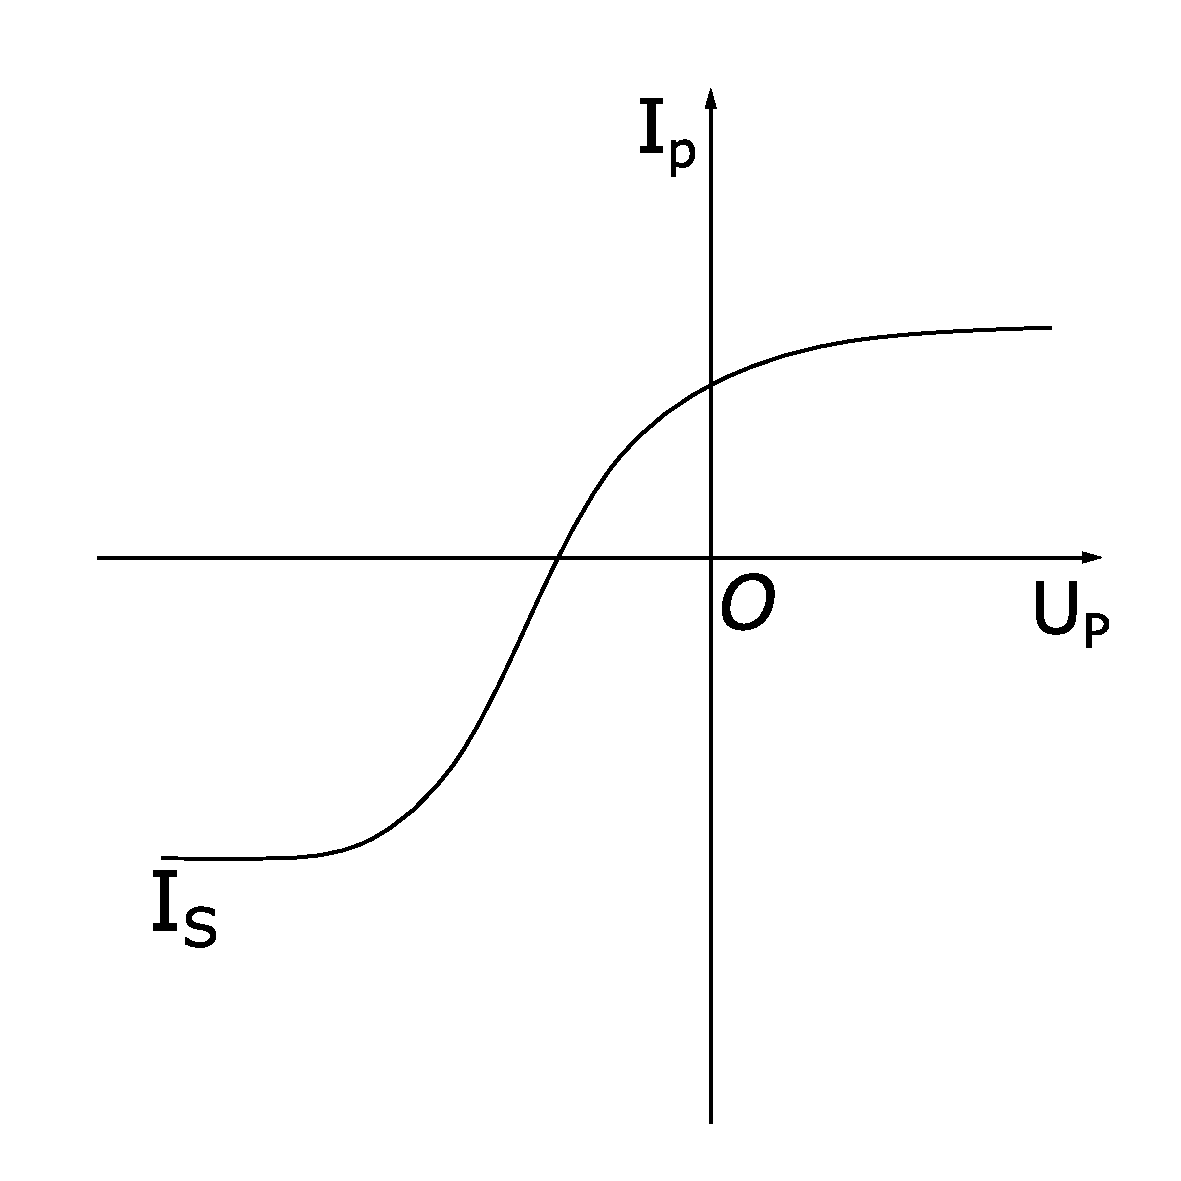
\includegraphics[width=0.4\textwidth]{fig/fig5.pdf}\\
\caption{双探针伏安特性}\label{fig5}
\end{figure}

在坐标原点,如果两根探针之间没有电位差,它们各自得到的电流相等,所以外电流为零。然而,一般说来,由于两个探针所在的等离子体电位稍有不同,所以外加电压为零时,电流不是零。

随着外加电压逐步增加,电流趋于饱和。最大电流是饱和离子电流$I_{s1}$、$I_{s2}$。

双探针法有一个重要的优点,即流到系统的总电流决不可能大于饱和离子电流。这是因为流到系统的电子电流总是与相等的离子电流平衡。从而探针对等离子体的干扰大为减小。

由双探针特性曲线,通过下式可求得电子温度$T_e$:
\begin{equation}
T_e = \cfrac{e}{k_B}\cfrac{I_{i1}I_{i2}}{I_{i1}+I_{i2}}\cfrac{\text{d}U}{\text{d}I}|_{U=0}\label{eq10}
\end{equation}
式中$I_{i1}$和$I_{i2}$为流到探针1和2的正离子电流。它们由饱和离子流确定。$\frac{\text{d}U}{\text{d}I}|_{U=0}$是U=0附近伏安特性曲线斜率。

电子密度$n_e$为:
\begin{equation}
n_e = \cfrac{2I_s}{eS}\sqrt{\cfrac{M}{k_BT_e}}\label{eq11}
\end{equation}
式中M是放电管所充气体的离子质量,S是两根探针的平均表面积。$I_s$是正离子饱和电流。

由双探针法可测定等离子体内的轴向电场强度$E_L$。一种方法是分别测定两根探针所在处的等离子体电位$U_1$和$U_2$,得
\begin{equation}
E_L = \cfrac{U_1 - U_2}{l}\label{eq12}
\end{equation}
式中$l$为两探针间距。

另一种方法称为补偿法,接线如图(\ref{fig6})所示。
\begin{figure}[!h]
\centering
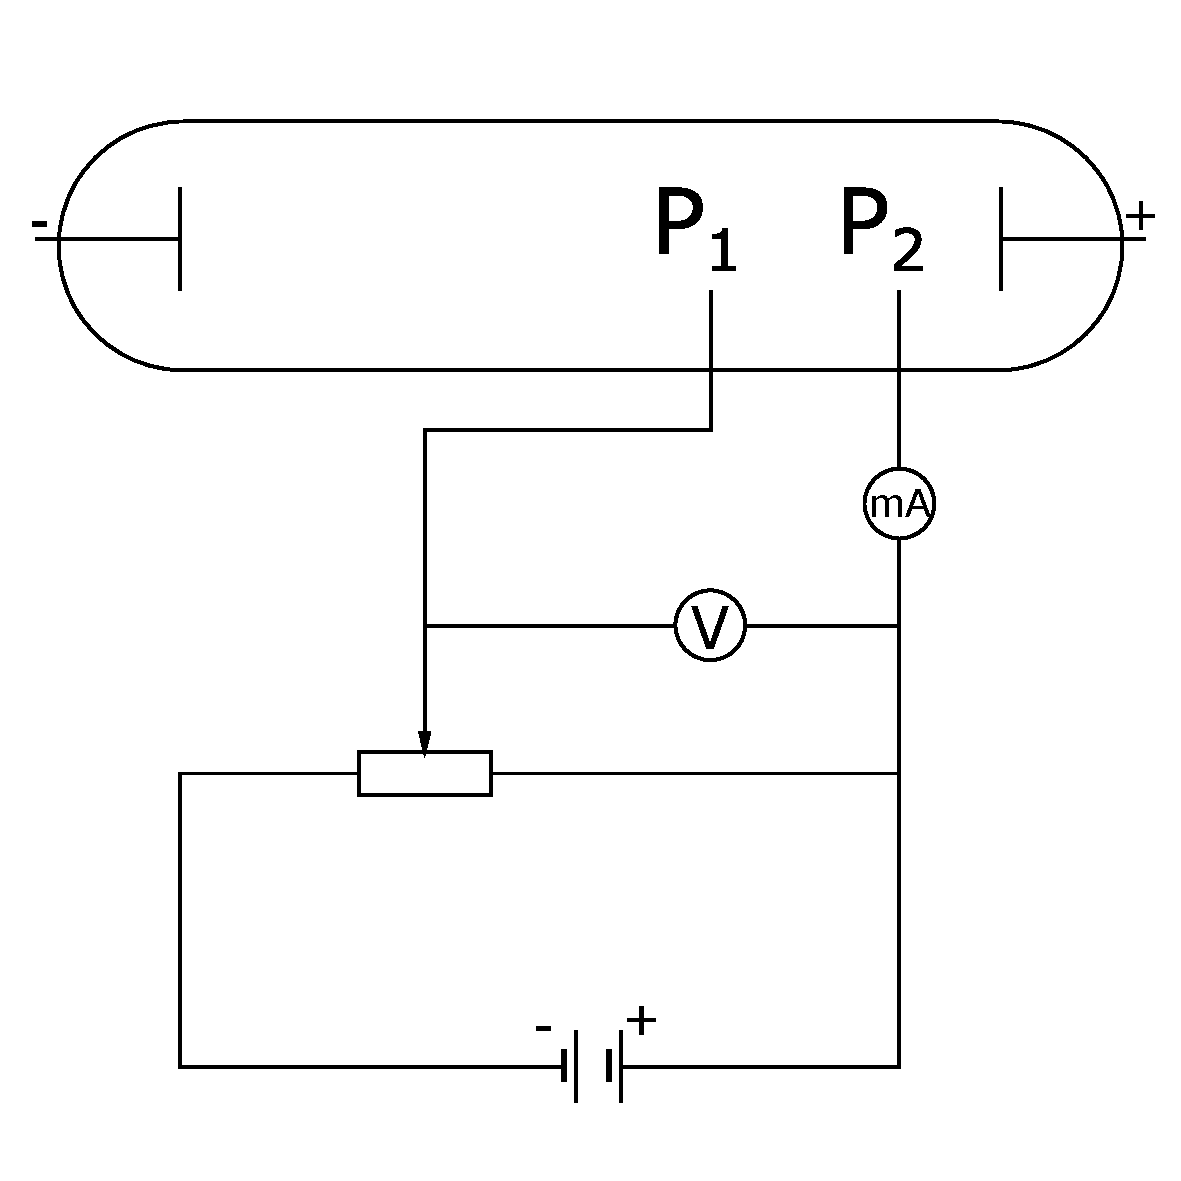
\includegraphics[width=0.4\textwidth]{fig/fig6.pdf}\\
\caption{补偿法接线}\label{fig6}
\end{figure}

当电流表上得读数为0时,伏特表上得电位差除以探针间距$l$,也可以得到$E_L$。

\section{实验内容}
\subsection{单探针法测等离子体参量}
本实验采用的是电脑化X-Y记录仪和等离子体实验辅助分析软件,测量伏安特性曲线,算出等离子体参量。

连好线路后接通电源,使放电管放电,将放电电流调到需要值,接通X-Y函数记录仪电源,选择合适的量程。在接线板上选择合适的取样电阻。运行电脑化X-Y记录仪数据采集软件,随着探针电位自动扫描,电脑自动描出U-I特性曲线,将数据保存。

用等离子体实验辅助分析软件处理数据,求得电子温度等主要参量。
\subsection{双探针法}
用自动记录法测出双探针伏安特性曲线,求$T_e$和$n_e$。
双探针法实验方法与单探针法相同。值得注意的是双探针法探针电流比单探针小两个数量级,故要选择合适的仪表量程。

\section{实验数据}
\begin{figure}[!h]
\centering
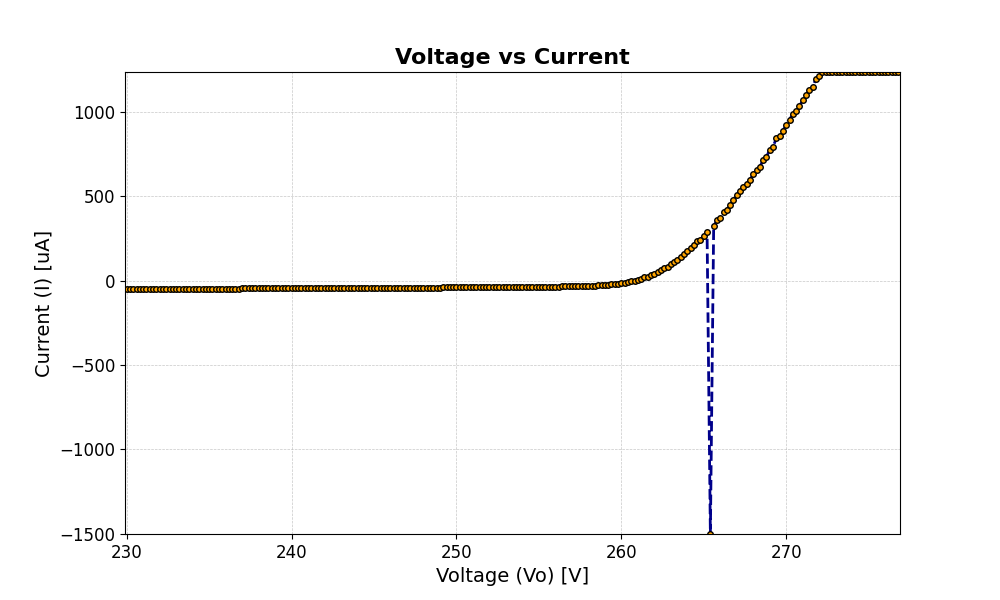
\includegraphics[width=0.6\textwidth]{data/Figure_1.png}\\
\caption{单探针法数据}\label{fig7}
\end{figure}

\begin{figure}[!h]
\centering
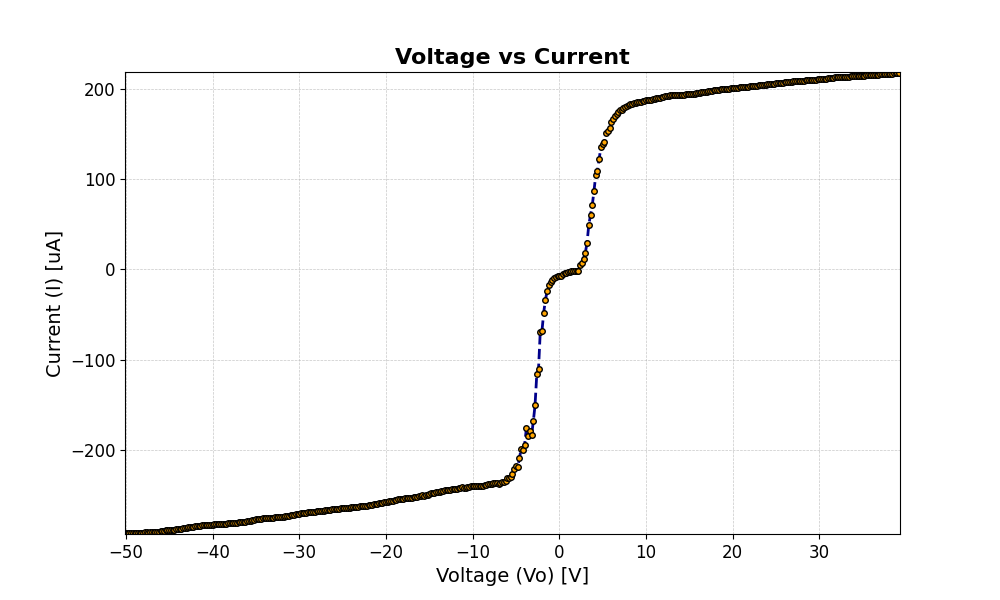
\includegraphics[width=0.6\textwidth]{data/Figure_2.png}\\
\caption{双探针法数据}\label{fig8}
\end{figure}

\begin{figure}[!h]
\centering
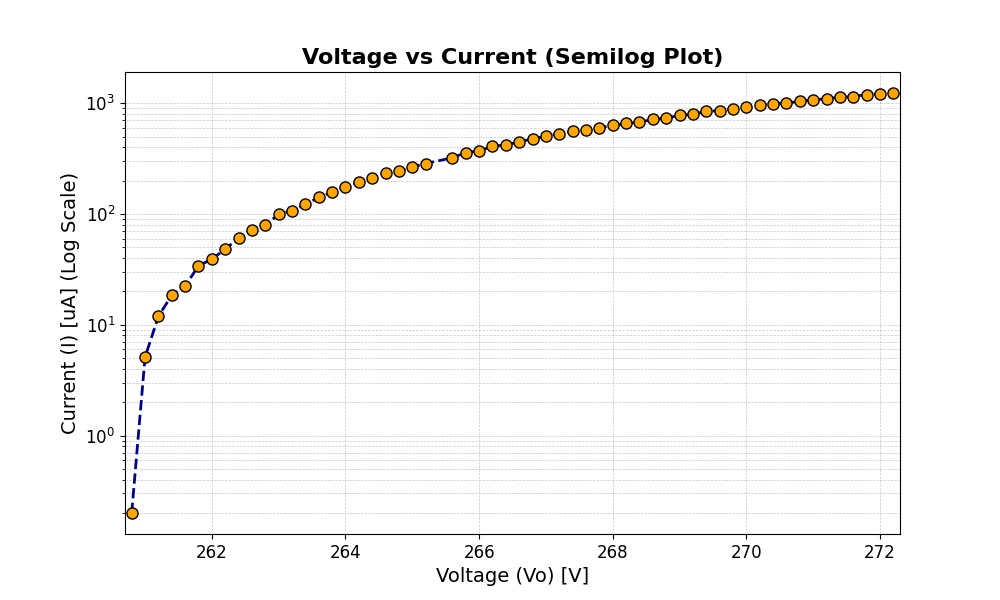
\includegraphics[width=0.6\textwidth]{data/Figure_1_2.png}\\
\caption{单探针法半对数图}\label{fig9}
\end{figure}
将单探针法和双探针法得到的数据绘图,分别得到图\ref{fig7} 和图\ref{fig8}。下面将对两种方法得到的数据分别进行从处理,得到电子温度$T_{e}$和电子密度$n_{e}$。

处理单探针法得到的数据,作半对数图,得到图\ref{fig9}。计算得到$\tan\phi=0.8452$,$T_{e}=13724K$,在$10^{4}$量级。
为了求等离子区的电子密度,计算得到需要的$I_0=1234.9  \mu A$,$S=1.257\times 10^{-7}m^{2}$,计算得到电子密度$n_{e}=3.37\times 10^{17} m^{-3}$。

处理双探针法得到的数据,$I_{s1}$和$I_{s2}$分别为$292\mu A$和$218\mu A$,计算得到$T_{e}=43198K$,在$10^{4}$量级。计算得到电子密度$n_{e}=7.23\times 10^{18} m^{-3}$。
\section{误差分析}
单探针法和双探针法中都有来自于探针非理想形状和等离子体不稳定特点的偶然误差。双探针法和单探针法相比,克服了来自于等离子体自身电势差的系统误差。
\section{思考题}
\subsection{气体放电中的等离子体有什么特征?}
\begin{itemize}
    \item 高度电离,是电和热的良导体,具有比普通气体大几百倍的比热容;
    \item 带正电的和带负电的粒子密度几乎相等;
    \item 宏观上是电中性的。
\end{itemize}
\subsection{等离子体有哪些主要的参量?}
\begin{itemize}
    \item 电子温度$T_{e}$
    \item 带电粒子密度(电子密度/离子实密度)n
\end{itemize}
\subsection{探针法对探针有什么要求?}
\begin{itemize}
    \item 能够承受等离子管内的高温;
    \item 具有化学惰性,不与等离子管内物质反应;
    \item 对等离子体的干扰小。
\end{itemize}
\nocite{jiaocai}
\bibliography{ref}
\end{document}